\subsection{Implementace polymorfizmu (pozdní vazba, VMT)}

\begin{frame}[fragile]
\begin{bonusblock}{}
\vskip 2ex
\Large \centering
VMT (virtual method table)
\vskip 2ex
\end{bonusblock}
\end{frame}




\begin{frame}[fragile]
\begin{bonusblock}{VMT}
\begin{itemize}
\item VMT je vytvořena pro každou třídu, která obsahuje virtuální metody
\item ukazatel na VMT je automaticky vložen do každého objektu
\item VMT obsahuje:
\begin{itemize}
\item ukazatel na implementaci dané metody pro danou třídu
\item offset začátku objektu (viz problémy s vícenásobnou dědičností)
\end{itemize}
\end{itemize}
\end{bonusblock}

\begin{bonusblock}{Časná/pozdní vazba}
\begin{itemize}
\item při časné vazbě se kompilátor podívá na typ objektu a dosadí instrukci CALL s voláním příslušné metody
\item při pozdní vazbě kompilátor načte příslušný záznam z tabulky VMT (kterou má u sebe objekt) a zavolá zde definovanou metodu
\end{itemize}
\end{bonusblock}
\end{frame}




\begin{frame}[fragile]
\begin{yesblock}
\begin{twocols}
\begin{lstlisting}[basicstyle=\scriptsize]
struct A {
  virtual void method1() { }
  virtual void method2() { }

  int _a = 0xaaaaaaaa;
};
\end{lstlisting}
\twocolssep
\begin{lstlisting}[basicstyle=\scriptsize]
struct B : A {
  virtual void method1() override { }
  virtual void method2() override { }

  int _b = 0xbbbbbbbb;
};
\end{lstlisting}
\end{twocols}
\end{yesblock}
\pause
\begin{twocols}
\vskip 3ex
\begin{tabular}{c|c|l}
& objA & \\
\hline
0x00 & \grc \ttfamily $A_{vmt}$ & \\
\hline
0x04 & \ttfamily 0xaaaaaaaa & \\
\hline
\end{tabular}

\twocolssep

\begin{tabular}{c|c|l}
& \grc $A_{vmt}$ & \\
\hline
0x00 & \ttfamily A::method1 & \\
\hline
0x04 & \ttfamily A::method2 & \\
\hline
\end{tabular}
\end{twocols}
\pause
\begin{twocols}
\vskip 3ex
\begin{tabular}{c|c|l}
& objB & \\
\hline
0x00 & \bc \ttfamily $B_{vmt}$ & \\
\hline
0x04 & \ttfamily 0xaaaaaaaa & \\
\hline
0x08 & \ttfamily 0xbbbbbbbb &  \\
\hline
\end{tabular}

\twocolssep

\begin{tabular}{c|c|l}
& \bc $B_{vmt}$ & \\
\hline
0x00 & \ttfamily B::method1 & \\
\hline
0x04 & \ttfamily B::method2 & \\
\hline
\end{tabular}
\end{twocols}

\end{frame}






\begin{frame}[fragile]
\begin{yesblock}
\begin{lstlisting}[basicstyle=\small]
struct W {
  virtual void f() { } 
  virtual void g() { } 
  virtual void h() { } 
  virtual void k() { } 
}

struct AW : virtual W {
  virtual void g() override { }
}

struct BW : virtual W {
  virtual void h() override { }
}

struct CW : AW, BW {
  virtual void k() override { }
}

\end{lstlisting}
\end{yesblock}
\end{frame}





\begin{frame}[fragile]
\begin{twocols}

\begin{center}
\begin{tabular}{c|c|l}
& objCW & \\
\hline
 & \grc \ttfamily $ptr_{AW\rightarrow{}W}$ & $\leftarrow AW$ \\
\hline
 & \ttfamily AW data & \\
\hline
 & \ttfamily \ldots & \\
\hline
 & \grc \ttfamily $ptr_{BW\rightarrow{}W}$ & $\leftarrow BW$\\
\hline
 & \ttfamily BW data & \\
\hline
 & \ttfamily \ldots & \\
\hline
 & \ttfamily CW data & $\leftarrow CW$\\
\hline
 & \ttfamily \ldots & \\
\hline
 & \bc \ttfamily $CW_{vmt}$ & $\leftarrow W$\\
\hline
 & \ttfamily W data & \\
\hline
 & \ttfamily \ldots & \\
\hline
\end{tabular}
\end{center}
\twocolssep
\begin{center}
\begin{tabular}{c|c|l}
& \bc $CW_{vmt}$ & \\
\hline
0x00 & \ttfamily W::f & \\
\hline
0x04 & \ttfamily AW::g & \\
\hline
0x08 & \ttfamily BW::h & \\
\hline
0x0c & \ttfamily CW::k & \\
\hline
\end{tabular}
\end{center}
\end{twocols}
\end{frame}


\begin{frame}[fragile]
\frametitle{Realita dle MSVC 2017}
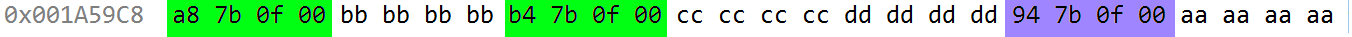
\includegraphics[width=\textwidth]{img/polymorfizmus2.png} \\
\vskip 1ex
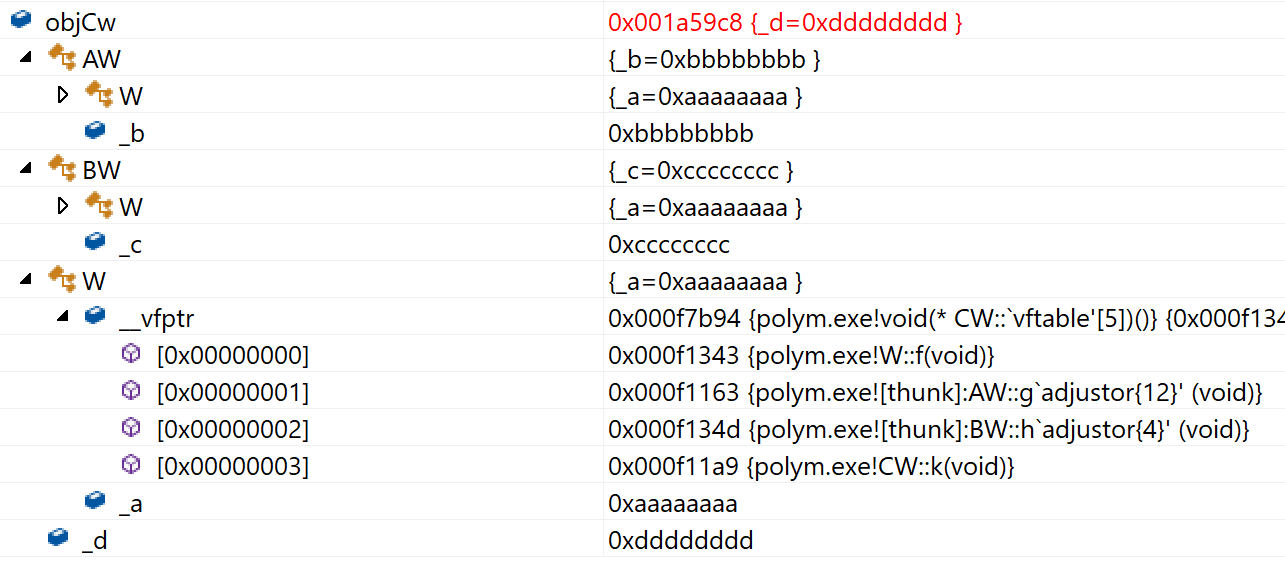
\includegraphics[width=\textwidth]{img/polymorfizmus.png}
\end{frame}

\zkouskove